\begin{frame}{Why Large-Scale ML?}
    \begin{columns}
        \begin{column}{0.6\textwidth}
            \begin{itemize}
                \item \textbf{Brawn or Brains?}
                \begin{itemize}
                    \item In 2001, Microsoft researchers ran a test to evaluate 4 different approaches to ML-based language translation
                \end{itemize}
                \item \textbf{Findings:}
                \begin{itemize}
                    \item Size of the dataset used to train the model mattered more than the model itself
                    \item As the dataset grew large, performance difference between the models became small
                \end{itemize}
            \end{itemize}
        \end{column}
        \begin{column}{0.4\textwidth}
            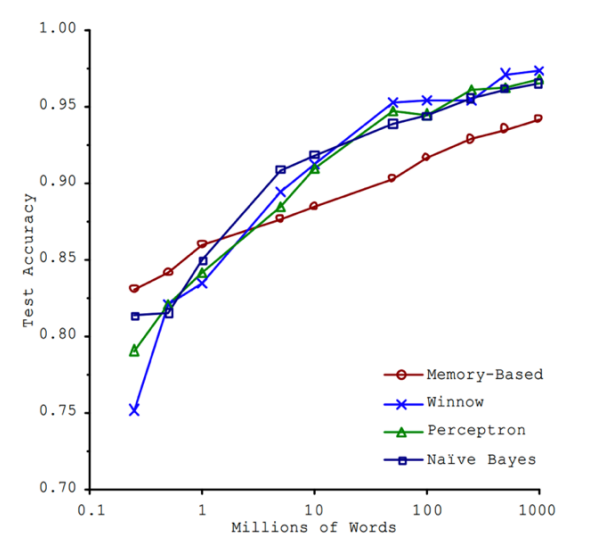
\includegraphics[width=\linewidth]{images/decision-trees/decision-trees-1.png}
        \end{column}
    \end{columns}

    \vspace{0.3cm}
    \tiny Banko, M. and Brill, E. (2001), ``\href{https://aclanthology.org/P01-1005/}{Scaling to Very Large Corpora for Natural Language Disambiguation}''
\end{frame}


\begin{frame}{Why Large-Scale ML?}
    \begin{columns}
        \begin{column}{0.6\textwidth}
            \begin{itemize}
                \item \textbf{The Unreasonable Effectiveness of Data}
                \begin{itemize}
                    \item In 2017, Google revisited the same type of experiment with the latest Deep Learning models in computer vision
                \end{itemize}
                \item \textbf{Findings:}
                \begin{itemize}
                    \item Performance increases logarithmically based on volume of training data
                    \item Complexity of modern ML models (i.e., deep neural nets) allows for even further performance gains
                \end{itemize}
                \item Large datasets + large ML models = amazing results!!
            \end{itemize}
        \end{column}
        \begin{column}{0.4\textwidth}
            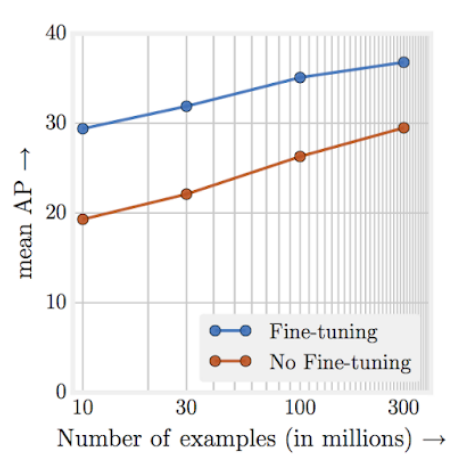
\includegraphics[width=\linewidth]{images/decision-trees/decision-trees-2.png}
        \end{column}
    \end{columns}

    \vspace{0.3cm}
    \tiny “Revisiting Unreasonable Effectiveness of Data in Deep Learning Era”: \href{https://arxiv.org/abs/1707.02968}{https://arxiv.org/abs/1707.02968}
\end{frame}


\begin{frame}{Why Worry About Non-Deep Models?}
            \begin{itemize}
                \item A few reasons why this is important:
                \item They outperform DL models in certain tasks.
                \item Deep models are often hard to scale and require lots of data. Traditional models allow you to encode prior knowledge better and give you more control.
                \item Combine: ideas from several ML models, e.g., GNNs
                \item Rule of thumb: If working on a well understood problem use deep learning. If working on a new problem use techniques we’ll discuss here.
            \end{itemize}
\end{frame}
